

\tikzset{every picture/.style={line width=0.75pt}} %set default line width to 0.75pt        

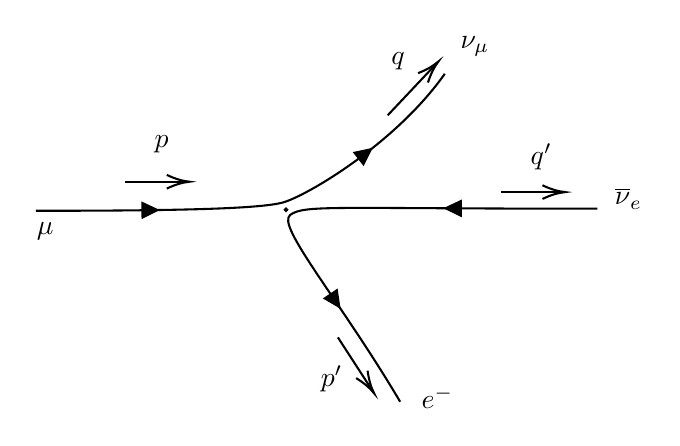
\begin{tikzpicture}[x=0.75pt,y=0.75pt,yscale=-1,xscale=1]
%uncomment if require: \path (0,300); %set diagram left start at 0, and has height of 300

%Curve Lines [id:da8199430993594923] 
\draw    (69.5,151) .. controls (139.5,151) and (177.5,150) .. (188.5,147) .. controls (199.5,144) and (242.5,119) .. (266.5,85) ;
\draw [shift={(129.26,150.63)}, rotate = 539.1700000000001] [fill={rgb, 255:red, 0; green, 0; blue, 0 }  ][line width=0.08]  [draw opacity=0] (8.93,-4.29) -- (0,0) -- (8.93,4.29) -- cycle    ;
\draw [shift={(231.84,120.65)}, rotate = 502.26] [fill={rgb, 255:red, 0; green, 0; blue, 0 }  ][line width=0.08]  [draw opacity=0] (8.93,-4.29) -- (0,0) -- (8.93,4.29) -- cycle    ;
%Curve Lines [id:da968566408247397] 
\draw    (245,243) .. controls (216,194) and (185,158) .. (192,153) .. controls (199,148) and (211,150) .. (340,150) ;
\draw [shift={(216.3,198.24)}, rotate = 236.02] [fill={rgb, 255:red, 0; green, 0; blue, 0 }  ][line width=0.08]  [draw opacity=0] (8.93,-4.29) -- (0,0) -- (8.93,4.29) -- cycle    ;
\draw [shift={(265.79,149.78)}, rotate = 0.32] [fill={rgb, 255:red, 0; green, 0; blue, 0 }  ][line width=0.08]  [draw opacity=0] (8.93,-4.29) -- (0,0) -- (8.93,4.29) -- cycle    ;
%Flowchart: Connector [id:dp043666729593928144] 
\draw  [color={rgb, 255:red, 0; green, 0; blue, 0 }  ,draw opacity=1 ][fill={rgb, 255:red, 0; green, 0; blue, 0 }  ,fill opacity=1 ] (190.5,150.5) .. controls (190.5,150.22) and (190.28,150) .. (190,150) .. controls (189.72,150) and (189.5,150.22) .. (189.5,150.5) .. controls (189.5,150.78) and (189.72,151) .. (190,151) .. controls (190.28,151) and (190.5,150.78) .. (190.5,150.5) -- cycle ;
%Straight Lines [id:da21277212072154672] 
\draw    (112.5,137) -- (141.5,137) ;
\draw [shift={(143.5,137)}, rotate = 180] [color={rgb, 255:red, 0; green, 0; blue, 0 }  ][line width=0.75]    (10.93,-3.29) .. controls (6.95,-1.4) and (3.31,-0.3) .. (0,0) .. controls (3.31,0.3) and (6.95,1.4) .. (10.93,3.29)   ;
%Straight Lines [id:da7169410729564696] 
\draw    (293.5,142) -- (322.5,142) ;
\draw [shift={(324.5,142)}, rotate = 180] [color={rgb, 255:red, 0; green, 0; blue, 0 }  ][line width=0.75]    (10.93,-3.29) .. controls (6.95,-1.4) and (3.31,-0.3) .. (0,0) .. controls (3.31,0.3) and (6.95,1.4) .. (10.93,3.29)   ;
%Straight Lines [id:da2318074943395163] 
\draw    (215,212) -- (231.41,237.32) ;
\draw [shift={(232.5,239)}, rotate = 237.05] [color={rgb, 255:red, 0; green, 0; blue, 0 }  ][line width=0.75]    (10.93,-3.29) .. controls (6.95,-1.4) and (3.31,-0.3) .. (0,0) .. controls (3.31,0.3) and (6.95,1.4) .. (10.93,3.29)   ;
%Straight Lines [id:da9531706570820151] 
\draw    (239,105) -- (262.13,80.46) ;
\draw [shift={(263.5,79)}, rotate = 493.3] [color={rgb, 255:red, 0; green, 0; blue, 0 }  ][line width=0.75]    (10.93,-3.29) .. controls (6.95,-1.4) and (3.31,-0.3) .. (0,0) .. controls (3.31,0.3) and (6.95,1.4) .. (10.93,3.29)   ;

% Text Node
\draw (74,161) node    {$\mu $};
% Text Node
\draw (130,119) node    {$p$};
% Text Node
\draw (244,79) node    {$q$};
% Text Node
\draw (212,232) node    {$p'$};
% Text Node
\draw (313,125) node    {$q'$};
% Text Node
\draw (281,72) node    {$\nu _{\mu }$};
% Text Node
\draw (263,241) node    {$e^{-}$};
% Text Node
\draw (355,145) node    {$\overline{\nu }_{e}$};


\end{tikzpicture}